\documentclass[preview]{standalone}

\usepackage{pgfplots}
\usepgfplotslibrary{fillbetween}
\usetikzlibrary{patterns}

\pgfplotsset{
  ticks=none,
  samples = 300
}

\begin{document}
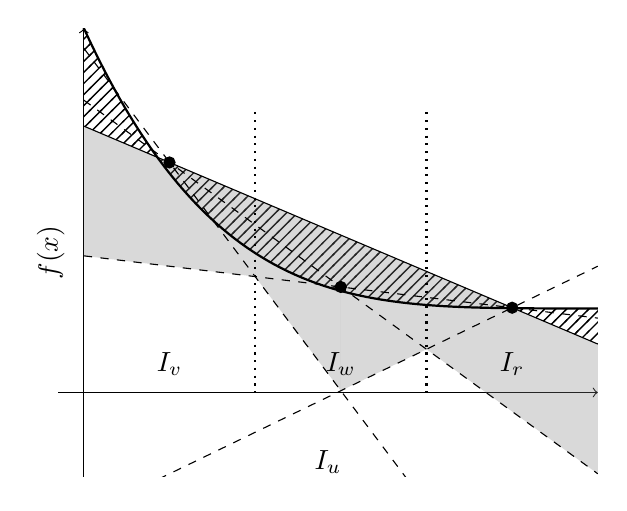
\begin{tikzpicture}
    \tikzset{
        hatch distance/.store in=\hatchdistance,
        hatch distance=10pt,
        hatch thickness/.store in=\hatchthickness,
        hatch thickness=2pt
    }

    \makeatletter
    \pgfdeclarepatternformonly[\hatchdistance,\hatchthickness]{flexible hatch}
    {\pgfqpoint{0pt}{0pt}}
    {\pgfqpoint{\hatchdistance}{\hatchdistance}}
    {\pgfpoint{\hatchdistance-1pt}{\hatchdistance-1pt}}%
    {
        \pgfsetcolor{\tikz@pattern@color}
        \pgfsetlinewidth{\hatchthickness}
        \pgfpathmoveto{\pgfqpoint{0pt}{0pt}}
        \pgfpathlineto{\pgfqpoint{\hatchdistance}{\hatchdistance}}
        \pgfusepath{stroke}
    }


  \begin{axis}[enlargelimits=0.1,xmin=-0.05,xmax = 1.0, ymin=-0.3,ymax=1.3,
    axis lines=middle,
    axis line style={->},
    x label style={at={(axis description cs:0.5,0.08)},anchor=north},
    y label style={at={(axis description cs:0.03,0.5)},rotate=90,anchor=south},
    xlabel={$I_u$},
    ylabel={$f(x)$}
    ]

    \addplot[name path=test,black,smooth,thick,domain=-0.1:1.1,samples=100]{0.3 + (1 - x)^4};

      \addplot[name path=phat,domain=0:1,black] {-0.777779*x + 0.950618};
      \addplot[name path=v2,domain=0:1,black,dashed] {-1.33334*x + 1.04321};
      \addplot[name path=r1,domain=0:1,black,dashed] {-0.22222*x + 0.487654};

      \addplot[name path=r2,domain=0:1,black,dashed] {0.888918*x - 0.438296};
      \addplot[name path=v1,domain=0:1,black,dashed] {-2.44444*x + 1.2284};
      
      \addplot +[mark=none,black,dotted,thick] coordinates {(0.33333, 1) (0.33333, 0)};
      \addplot +[mark=none,black,dotted,thick] coordinates {(0.66666, 1) (0.66666, 0)};
      \addplot [
      pattern=flexible hatch,
      hatch distance=5pt,
      hatch thickness=0.5pt,
      pattern color=black
      ]
      fill between[
      of=test and phat,
      soft clip={domain=0.0:1.0},
      ];

      \addplot [
      thick,
      color=gray,
      fill=gray,
      fill opacity=0.3
      ]
      fill between[
      of=r1 and phat,
      soft clip={domain=0.0:0.3333},
      ];

      \addplot [
      thick,
      color=gray,
      fill=gray,
      fill opacity=0.3
      ]
      fill between[
      of=v1 and phat,
      soft clip={domain=0.3333:0.5},
      ];
      \addplot [
      thick,
      color=gray,
      fill=gray,
      fill opacity=0.3
      ]
      fill between[
      of=r2 and phat,
      soft clip={domain=0.5:0.6666},
      ];

      \addplot [
      thick,
      color=gray,
      fill=gray,
      fill opacity=0.3
      ]
      fill between[
      of=v2 and phat,
      soft clip={domain=0.6666:1.0},
      ];
      
      
      \node at (axis cs: 0.166666, 0.1) {$I_v$};
      \node at (axis cs: 0.500000, 0.1) {$I_w$};
      \node at (axis cs: 0.833333, 0.1) {$I_r$};

      \addplot[only marks] table {
        0.166666 0.820988
        0.500000 0.376543
        0.833333 0.302469
      };
    \end{axis}
\end{tikzpicture}
\end{document}